%
% File eacl2017.tex
%

\documentclass[11pt]{article}
\usepackage{eacl2017}
\usepackage{times}
\usepackage{url}
\usepackage{latexsym}
\usepackage{times}
\usepackage{url}
\usepackage{amsmath}
\usepackage{breqn}
\usepackage{latexsym}
\usepackage{pgfplotstable}
\usepackage{algorithm2e}
\usepackage{hhline}
\usepackage{multirow}
\usepackage[font=small]{caption}
\usepackage{subcaption}
%\usepackage{hyperref}
\usepackage{color}
\usepackage{lipsum,adjustbox}
\usepackage{tikz}
\usepackage{tikz-dependency}
\usetikzlibrary{shapes,fit,calc,er,positioning,intersections,decorations.shapes,mindmap,trees}
\tikzset{decorate sep/.style 2 args={decorate,decoration={shape backgrounds,shape=circle,
      shape size=#1,shape sep=#2}}}
\newcommand{\oa}[1]{\footnote{\color{red} #1}}
\newcommand{\daniel}[1]{\footnote{\color{blue} #1}}
\newcommand{\com}[1]{}
\newcommand{\parser}[1]{TUPA\textsubscript{#1}}
\newcommand{\secref}[1]{Section~\ref{#1}}
\newcommand{\figref}[1]{Figure~\ref{#1}}
\newcommand{\tabref}[1]{Table~\ref{#1}}
\DeclareMathOperator*{\argmin}{argmin}
\DeclareMathOperator*{\argmax}{argmax}
\SetKwRepeat{Do}{do}{while}
\renewcommand\AlCapFnt{\normalfont\small}
\hyphenation{SemEval}

%\eaclfinalcopy % Uncomment this line for the final submission
%\def\eaclpaperid{***} %  Enter the acl Paper ID here

%\setlength\titlebox{5cm}
% You can expand the titlebox if you need extra space
% to show all the authors. Please do not make the titlebox
% smaller than 5cm (the original size); we will check this
% in the camera-ready version and ask you to change it back.

\title{Broad-Coverage Transition-Based UCCA Parsing}

\author{Daniel Hershcovich$^{1,2}$ \And Omri Abend$^2$ \And Ari Rappoport$^2$ \\
  $^1$Edmond and Lily Safra Center for Brain Sciences, Hebrew University of Jerusalem \\
  $^2$School of Computer Science and Engineering, Hebrew University of Jerusalem \\
  \texttt{\{danielh,oabend,arir\}@cs.huji.ac.il}
}

\date{}

\begin{document}
\maketitle

%%%%%%%%%%%%%%%%%%%%%%%%%%%%%%%%%%%%%%%%%%%%%%%%%%%%%%%%%%%%%%%
%%%%%%%%%%%%%%%%%     Abstract     %%%%%%%%%%%%%%%%%%%%%%%%%%%%
%%%%%%%%%%%%%%%%%%%%%%%%%%%%%%%%%%%%%%%%%%%%%%%%%%%%%%%%%%%%%%%
\begin{abstract}
  We present the first parser for UCCA, a
  cross-linguistically applicable framework for semantic
  representation, that builds on extensive
  typological work, and supports rapid annotation.
  UCCA poses a challenge for existing parsing techniques,
  as it exhibits reentrancy (resulting in DAG structures),
  discontinuous structures and non-terminal nodes corresponding
  to complex semantic units. To our knowledge, the conjunction
  of these formal properties is not supported by any existing parser.
  Our transition-based parser, using novel transition set
  and features, has value not just for UCCA parsing:
  its ability to handle more general graph structures will inform
  the development of parsing methods into other semantic DAG structures, 
  and parsing in languages which frequently use discontinuous structures.
\end{abstract}


%%%%%%%%%%%%%%%%%%%%%%%%%%%%%%%%%%%%%%%%%%%%%%%%%%%%%%%%%%%%%%%
\section{Introduction}\label{sec:introduction}

Universal Conceptual Cognitive Annotation, (UCCA, \newcite{abend2013universal}),
is a cross-linguistically applicable semantic representation scheme,
building on the established Basic Linguistic Theory typological framework
\cite{Dixon:10b,Dixon:10a,Dixon:12}, and on Cognitive
Linguistics literature \cite{croft2004cognitive}.
UCCA has demonstrated applicability to multiple languages, including
English, French, German and Czech, support for rapid annotation,
and semantic stability in translation \cite{sulem2015conceptual}.
The scheme has proven useful for machine translation evaluation \cite{birch2016hume},
but its applicability has been so far limited by the absence of a UCCA parser,
a gap this paper addresses.

Formally, a UCCA structure is a DAG whose leaves correspond to the tokens of
the text. Nodes (or {\it units}) either correspond to a terminal or
to several sub-units (not necessarily contiguous) jointly viewed as a
single entity according to some semantic or cognitive consideration.
Edges bear a category, indicating the role of the sub-unit in the relation
that the parent represents. \figref{fig:examples} presents a few UCCA-annotated examples.

\begin{figure}[t]
  \begin{subfigure}[t]{.9\columnwidth}
  \parbox{.1\columnwidth}{\caption{}\label{fig:graduation}}
  \parbox{.8\columnwidth}{
  \scalebox{.9}{
  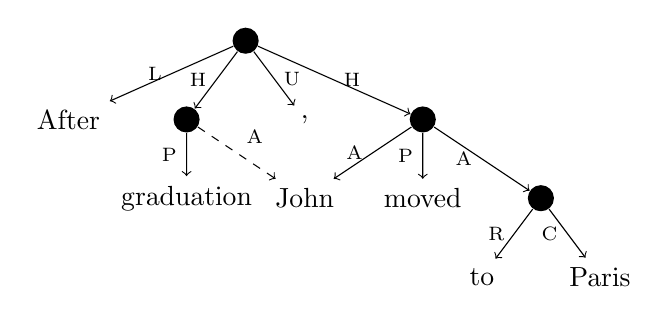
\begin{tikzpicture}[level distance=10mm, ->,
      every circle node/.append style={fill=black}]
    \node (ROOT) [circle] {}
      child {node (After) {After} edge from parent node[left] {\scriptsize L}}
      child {node (graduation) [circle] {}
      {
        child {node {graduation} edge from parent node[left] {\scriptsize P}}
      } edge from parent node[left] {\scriptsize H} }
      child {node {,} edge from parent node[right] {\scriptsize U}}
      child {node (moved) [circle] {}
      {
        child {node (John) {John} edge from parent node[left] {\scriptsize A}}
        child {node {moved} edge from parent node[left] {\scriptsize P}}
        child {node [circle] {}
        {
          child {node {to} edge from parent node[left] {\scriptsize R}}
          child {node {Paris} edge from parent node[left] {\scriptsize C}}
        } edge from parent node[left] {\scriptsize A} }
      } edge from parent node[right] {\scriptsize H} }
      ;
    \draw[dashed,->] (graduation) to node [auto] {\scriptsize A} (John);
  \end{tikzpicture}
  }}
  \end{subfigure}
  \begin{subfigure}[t]{.9\columnwidth}
  \parbox{.1\columnwidth}{\caption{}\label{fig:gave}}
  \hspace{.25\columnwidth}
  \parbox{.55\columnwidth}{
  \scalebox{.9}{
  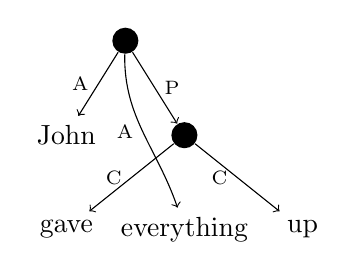
\begin{tikzpicture}[level distance=12mm, ->,
      every node/.append style={midway},
      every circle node/.append style={fill=black}]
    \node (ROOT) [circle] {}
      child {node {John} edge from parent node[left] {\scriptsize A}}
      child {node [circle] {}
      {
      	child {node {gave} edge from parent node[left] {\scriptsize C}}
      	child {node (everything) {everything} edge from parent[white]}
      	child {node {up} edge from parent node[left] {\scriptsize C}}
      } edge from parent node[right] {\scriptsize P} }
      ;
    \draw[bend right,->] (ROOT) to[out=-20, in=180] node [left] {\scriptsize A} (everything);
  \end{tikzpicture}
  }}
  \end{subfigure}
  \begin{subfigure}[t]{.9\columnwidth}
  \parbox{.1\columnwidth}{\caption{}\label{fig:home}}
  \hspace{.1\columnwidth}
  \parbox{.7\columnwidth}{
  \scalebox{.9}{
  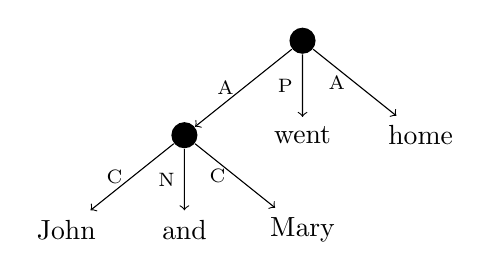
\begin{tikzpicture}[level distance=12mm, ->,
      every node/.append style={midway},
      every circle node/.append style={fill=black}]
    \node (ROOT) [circle] {}
      child {node [circle] {}
      {
        child {node {John} edge from parent node[left] {\scriptsize C}}
        child {node {and} edge from parent node[left] {\scriptsize N}}
        child {node {Mary} edge from parent node[left] {\scriptsize C}}
      } edge from parent node[left] {\scriptsize A} }
      child {node {went} edge from parent node[left] {\scriptsize P}}
      child {node {home} edge from parent node[left] {\scriptsize A}}
      ;
  \end{tikzpicture}
  }}
  \end{subfigure}
  \caption{\label{fig:examples}
    UCCA structures demonstrating three structural properties exhibited by
    the scheme.
    (\subref{fig:graduation}) includes a remote edge (dashed),
    resulting in ``John'' having two parents.
    (\subref{fig:gave}) includes a discontinuous unit (``gave ... up'').
    (\subref{fig:home}) includes a coordination construction (``John and Mary'').
    Legend: $P$ -- process (a scene's main relation), $A$ -- participant,
    $L$ -- inter-scene linker, $H$ -- linked scene, $C$ -- center,
    $R$ -- relator, $N$ -- connector, $U$ -- punctuation, $F$ -- function unit.
    Pre-terminal nodes are omitted for brevity.
  }
\end{figure}

Alongside recent progress in dependency parsing into projective trees
\cite{dyer2015transition,andor2016globally,kiperwasser2016simple},
there is increasing interest in broad-coverage parsing
(see \secref{sec:related_work}),
directed at representations supporting more general structural properties.
One such property is \textbf{reentrancy},
referring to arguments and relations (semantic units) that are shared between predicates.
For instance, in the sentence
``After graduation, John moved to Paris'' (\figref{fig:graduation}),
``John'' is an argument of both ``graduation''
and ``moved'', yielding a UCCA structure that is a DAG rather than a tree.

A second property is \textbf{discontinuity} (similar to \textit{non-projectivity} in bilexical schemes), as in ``John \textit{gave} everything \textit{up}''
(\figref{fig:gave}), where ``gave up'' forms a discontinuous semantic unit.
Discontinuities are pervasive, e.g.,  with multi-word
expressions \cite{schneider2014discriminative}.

Finally, UCCA uses \textbf{non-terminal nodes}
to represent units comprising more than one word.
The use of non-terminal nodes is motivated by constructions that have no clear head, including
coordination structures (e.g., ``\textit{John and Mary} went home''; \figref{fig:home}),
some multi-word expressions (e.g., ``The Haves and the \textit{Have Nots}''),
and prepositional phrases.

No existing parser, to our knowledge, supports the three structural properties described above.
We propose \parser{} (Transition-based UCCA Parser), taking a transition-based approach.
Building on existing knowledge in tackling these three properties
in isolation, we define an extended set of transitions and features
that supports reentrancy, discontinuities and non-terminal nodes.

Transition-based techniques are a natural
starting point for UCCA parsing, given the conceptual similarity of UCCA's distinctions,
centered around predicate-argument structures, to distinctions expressed by dependency schemes.
We are further motivated by the strength of transition-based methods
in similar tasks, including syntactic dependency parsing
\cite{dyer2015transition,andor2016globally,kiperwasser2016simple},
discontinuous syntactic constituency parsing \cite{maier-lichte:2016:DiscoNLP},
AMR parsing \cite{wang2015transition,wang-EtAl:2016:SemEval}
and CCG parsing \cite{ambati2015incremental,ambati-deoskar-steedman:2016:N16-1},
as well as joint lexical and syntactic parsing
\cite{constant-nivre:2016:P16-1}.

We evaluate \parser{} on the available English UCCA corpora, in both
in-domain and out-of-domain settings (\secref{sec:exp_setup}).
As a point of comparison, we assess the ability of existing bilexical DAG
parsers to tackle the task, by developing a conversion protocol
between UCCA and bilexical graphs.
Results show superior accuracy for \parser{}, demonstrating the effectiveness of
the approach for UCCA parsing (\secref{sec:results}),
and suggest concrete paths for further improvement (\secref{sec:discussion})
All converters and parsers will be made publicly available upon publication.


%%%%%%%%%%%%%%%%%%%%%%%%%%%%%%%%%%%%%%%%%%%%%%%%%%%%%%%%%%%%%%%
\section{The UCCA Scheme}\label{sec:ucca}

UCCA is a multi-layered representation, each layer corresponding
to a ``module'' of semantic distinctions.
The UCCA foundational layer, which we target in this paper, covers the predicate-argument
structure evoked by predicates of all grammatical categories
(verbal, nominal, adjectival and others), the inter-relations between them,
and other major linguistic phenomena such as coordination and multi-word expressions.

The layer's basic notion is the {\it Scene}, describing a movement, action or state.
Each Scene contains one main relation (marked as either a Process or a State),
as well as one or more Participants.
For example, the sentence ``After graduation, John moved to Paris'' (\figref{fig:graduation})
contains two Scenes, whose main relations are ``graduation'' and ``moved''.
``John'' is a Participant in both Scenes, while ``Paris'' only in the latter.
One incoming edge for each non-root node is marked as ``primary'',
and the rest (mostly denoting implied relations) as ``remote'' edges.
This distinction is made by the annotator.
The primary edges thus form a tree structure, whereas the remote edges enable reentrancy.

Further categories account for relations between Scenes and the internal structure of
complex arguments and relations (e.g. coordination; complex
adverbials such as ``very clearly'').
%\footnote{All UCCA-related resources can be found here:
%  \url{http://www.cs.huji.ac.il/~oabend/ucca.html}.}


%%%%%%%%%%%%%%%%%%%%%%%%%%%%%%%%%%%%%%%%%%%%%%%%%%%%%%%%%%%%%%%
\section{Broad-Coverage UCCA Parsing}\label{sec:direct_approach}

We now turn to presenting \parser{},
a transition-based parser supporting the structural properties of UCCA.
Transition-based parsers \cite{Nivre03anefficient} scan the text from start to end,
and create the parse incrementally by applying a \textit{transition}
at each step to the parser state,
defined using three data structures: a buffer $B$ of tokens and nodes to be processed,
a stack $S$ of nodes currently being processed,
and a graph $G=(V,E,\ell)$ of constructed nodes and edges,
where $V$ is the set of \emph{nodes}, $E$ is the set of \emph{edges},
and $\ell : E \to L$ is the \emph{label} function, $L$ being the set of possible labels.
Some of the states are marked as \textit{terminal}, meaning that $G$ is the final output.
A classifier is used at each step to select the next transition based on features
encoding the parser's current state.
During training, an oracle creates training instances for the classifier,
based on gold-standard annotations.

Transition-based methods have yielded excellent
results in a variety of parsing tasks.
Within syntactic dependency parsing, transition-based methods
have been successfully applied to corpora in many languages and domains, yielding
the best reported results for English
\cite{dyer2015transition,andor2016globally,kiperwasser2016simple}.
The approach has further yielded results comparable with the state-of-the-art in
constituency parsing \cite{sagae2005classifier,zhang2009transition,zhu2013fast},
discontinuous constituency parsing \cite{maier2015discontinuous,maier-lichte:2016:DiscoNLP},
as well as dependency DAG structures
\cite{sagae2008shift,ribeyre-villemontedelaclergerie-seddah:2014:SemEval,tokgoz2015transition}, CCG \cite{ambati2015incremental,ambati-deoskar-steedman:2016:N16-1,dipendra2016neural}\oa{is Misra and Artzi a CCG parser or a semantic parser that uses CCG?} and AMR parsing \cite{wang2015transition,wang-EtAl:2016:SemEval}.

\parser{} mostly builds on recent advances in discontinuous constituency
and dependency DAG parsing, and further introduces novel features for UCCA.

\paragraph{Transition Set.}
Given a sequence of tokens $w_1, \ldots, w_n$, we predict a UCCA graph $G$ over the sequence.
Parsing starts with a single node on the stack (an artificial root node), and the input tokens
in the buffer. The set of transitions is given in \figref{fig:transitions}.
In addition to the standard \textsc{Shift} and \textsc{Reduce} operations, 
we follow previous work in transition-based constituency parsing \cite{sagae2005classifier},
adding the \textsc{Node} transition for creating new non-terminal nodes.
\textsc{Node$_X$} creates a new node on the buffer as a parent of the first element on the stack, with an $X$-labeled edge.


\begin{figure*}
\begin{adjustbox}{width=\textwidth,margin=3pt,frame}
\begin{tabular}{llll|l|llllc|c}
\multicolumn{4}{c|}{\textbf{\small Before Transition}} & \textbf{\small Transition} & \multicolumn{5}{c|}{\textbf{\small After Transition}} & \textbf{\small Condition} \\
\textbf{\footnotesize Stack} & \textbf{\footnotesize Buffer} & \textbf{\footnotesize Nodes} & \textbf{\footnotesize Edges} & & \textbf{\footnotesize Stack} & \textbf{\footnotesize Buffer} & \textbf{\footnotesize Nodes} & \textbf{\footnotesize Edges} & \textbf{\footnotesize Terminal?} & \\
$S$ & $x \;|\; B$ & $V$ & $E$ & \textsc{Shift} & $S \;|\; x$ & $B$ & $V$ & $E$ & $-$ & \\
$S \;|\; x$ & $B$ & $V$ & $E$ & \textsc{Reduce} & $S$ & $B$ & $V$ & $E$ & $-$ & \\
$S \;|\; x$ & $B$ & $V$ & $E$ & \textsc{Node$_X$} & $S \;|\; x$ & $y \;|\; B$ & $V \cup \{ y \}$ & $E \cup \{ (y,x)_X \}$ & $-$ &
$x \neq \mathrm{root}$ \\
$S \;|\; y,x$ & $B$ & $V$ & $E$ & \textsc{Left-Edge$_X$} & $S \;|\; y,x$ & $B$ & $V$ & $E \cup \{ (x,y)_X \}$ & $-$ &
\multirow{4}{50pt}{\vspace{-5mm}\[\left\{\begin{array}{l}
x \not\in w_{1:n},\\
y \neq \mathrm{root},\\
y \not\leadsto_G x
\end{array}\right.\]} \\
$S \;|\; x,y$ & $B$ & $V$ & $E$ & \textsc{Right-Edge$_X$} & $S \;|\; x,y$ & $B$ & $V$ & $E \cup \{ (x,y)_X \}$ & $-$ & \\
$S \;|\; y,x$ & $B$ & $V$ & $E$ & \textsc{Left-Remote$_X$} & $S \;|\; y,x$ & $B$ & $V$ & $E \cup \{ (x,y)_X^* \}$ & $-$ & \\
$S \;|\; x,y$ & $B$ & $V$ & $E$ & \textsc{Right-Remote$_X$} & $S \;|\; x,y$ & $B$ & $V$ & $E \cup \{ (x,y)_X^* \}$ & $-$ & \\
$S \;|\; x,y$ & $B$ & $V$ & $E$ & \textsc{Swap} & $S \;|\; y$ & $x \;|\; B$ & $V$ & $E$ & $-$ &
$\mathrm{i}(x) < \mathrm{i}(y)$ \\
$[\mathrm{root}]$ & $\emptyset$ & $V$ & $E$ & \textsc{Finish} & $\emptyset$ & $\emptyset$ & $V$ & $E$ & $+$ & \\
\end{tabular}
\end{adjustbox}
\caption{\label{fig:transitions}
  The transition set of \parser{}. %Following standard practice,
  We write the stack with its top to the right and the buffer with its head to the left.
  $(\cdot,\cdot)_X$ denotes a primary $X$-labeled edge, and $(\cdot,\cdot)_X^*$ a remote $X$-labeled edge.
  $\mathrm{i}(x)$ is a running index for the created nodes.
  \textsc{Edge} transitions have an additional condition: the prospective child may not
  already have a primary parent.
}
\end{figure*}

\textsc{Left-Edge$_X$} and \textsc{Right-Edge$_X$} create a new primary $X$-labeled edge between the first two elements on the stack, where the parent is the left or the right node, respectively.
As a UCCA node may only have one incoming primary edge,
\textsc{Edge} transitions are disallowed if the child node already
has an incoming primary edge.
\textsc{Left-Remote$_X$} and \textsc{Right-Remote$_X$} do not have this restriction,
and the created edge is additionally marked as \textit{remote}.
We distinguish between these two pairs of transitions to allow the parser to create remote edges
without the possibility of producing invalid graphs.
To support the prediction of multiple parents, node and edge transitions
leave the stack unchanged, as in other work on
transition-based DAG dependency parsing
\cite{sagae2008shift,ribeyre-villemontedelaclergerie-seddah:2014:SemEval,tokgoz2015transition}.
Once all edges for a node have been created, it is removed from the stack
by applying \textsc{Reduce}.
To handle discontinuous nodes, \textsc{Swap} pops the second
node on the stack and adds it to the top of the buffer, as with the similarly
named transition in previous work \cite{nivre2009non,maier2015discontinuous}.
Finally, \textsc{Finish} pops the root node and marks the state as terminal.

\paragraph{Classifier.}
We experiment with three classifiers\footnote{A link to the code repository will
be released upon publication.}.
First, following \newcite{maier2015discontinuous} and \newcite{maier-lichte:2016:DiscoNLP},
we use a linear classifier, using sparse features and
the averaged structured perceptron algorithm for training it
\cite{Coll:04} with the \textsc{MinUpdate} procedure \cite{goldberg2011learning}:
a minimum number of updates to a feature has to occur in training for it
to be included in the model.
We refer to the parser using this classifier as \parser{sparse}.
Second, we experiment with a linear classifier using dense embedding features (see below),
which we also train using averaged structured perceptron.
We refer to this parser as \parser{dense}.
Third, we use a feedforward neural network, similar in architecture to that of \newcite{chen2014fast}, with the following modifications: two hidden layers instead of one, using the sigmoid activation function instead of cube,
and applying dropout after each layer \cite{srivastava2014dropout}.
We refer to the NN-based parser as \parser{NN}.

For all classifiers, inference is performed greedily, i.e., without beam search.

\paragraph{Features.}
For the sparse perceptron-based parser (\parser{sparse}),
we use binary indicator features representing
the word, POS tags and existing edge labels related to the top four stack elements and the next
three buffer elements, in addition to their children and grandchildren in the graph.
We also use bi- and trigram features based on these values \cite{zhang2009transition,zhu2013fast},
features related to discontinuous nodes adopted from \cite{maier2015discontinuous},
and features representing existing edges and the number of parents and children a node has, following \cite{tokgoz2015transition}.
In addition, we use novel, UCCA-specific features related to remote edges\footnote{See
supplementary material for a full listing of the feature templates.}.

For the dense perceptron-based (\parser{dense}) and the NN-based parser (\parser{NN}),
we replace all binary features by a
concatenation of the vector embeddings of all the represented elements:
words, POS tags, edge labels and parser actions.

Finally, for all classifiers we employ a real-valued feature,
\textbf{ratio}, corresponding to the ratio between the number of terminals to number of nodes
in the graph $G$.
This novel feature serves as a regularizer for the creation of new nodes,
and should be beneficial for other transition-based constituency parsers too.

\paragraph{Training.}
For training the transition classifier, we use a dynamic oracle \cite{goldberg2012dynamic},
i.e., an oracle that outputs a set of optimal transitions: when
applied to the current parser state, the gold
standard graph is reachable from the resulting state.
For example, the oracle would predict a \textsc{Node} transition if the stack 
has on its top a parent in the gold graph that has not been created,
but would predict a \textsc{Right-Edge} transition if the second stack
element is a parent of the
first element according to the gold graph and the edge between them has not been created.
The transition predicted by the classifier is deemed correct
and is applied to the parser state to reach the subsequent state,
if the transition is included in the set of optimal transitions.
Otherwise, a random optimal transition is applied,
and for the perceptron-based parser, the classifier's weights are updated according
to the perceptron update rule.

We train the perceptron classifiers for 16 iterations, using $\textsc{MinUpdate}=5$
and $\textsc{Importance}=2$, doubling weight updates
for gold \textsc{Swap} transitions to address the sparsity of discontinuous nodes,
as in \newcite{maier2015discontinuous}.
POS tags are extracted using the averaged perceptron tagger of NLTK \cite{bird2009natural}.
Word embeddings for the dense perceptron are initialized with the 100-dimensional pre-trained word2vec vectors \cite{mikolov2013efficient},
the same ones used by \newcite{dyer2015transition}\footnote{
\url{https://github.com/clab/lstm-parser}}.

For the NN classifier, the word embeddings are initialized to random
100-dimensional vectors (which were found to give better results than the pre-trained vectors). We use 1000-dimensional hidden layers.
For both the dense perceptron and the NN classifiers, we initialize the POS tag embeddings to random 20-dimensional vectors. The embeddings for existing edge labels are 10-dimensional, and for parser actions are 5-dimensional.
We use the categorical cross-entropy objective function and train the
NN classifier with the Adam optimizer \cite{kingma2014adam}. We use a dropout probability of 0.2,
and train the network for 50 epochs on a batch of 100 sentences at a time.
We use the Keras package \cite{chollet2015keras} for implementing the NN classifier.

%%%%%%%%%%%%%%%%%%%%%%%%%%%%%%%%%%%%%%%%%%%%%%%%%%%%%%%%%%%%%%%
\section{Experimental Setup}\label{sec:exp_setup}

\paragraph{Data.}
We conduct our main experiments on the UCCA Wikipedia corpus (henceforth, \textit{Wiki}),
and use the English part of the UCCA \textit{Twenty Thousand Leagues Under the Sea} English-French parallel corpus (henceforth, \textit{20K Leagues}) as
out-of-domain data.\footnote{Both are available at \url{http://www.cs.huji.ac.il/~oabend/ucca.html}}
\tabref{table:data} presents some statistics for the two corpora, demonstrating that while
the \textit{Wiki} corpus is over ten times larger, the overall statistics are
similar.
We use passages of indices up to 675
of the \textit{Wiki} corpus as our training set, passages 676--807 as development set,
and passages 808--1028 as in-domain test set.
While UCCA edges can cross sentence boundaries, we adhere to the common
practice in semantic parsing and train our parsers on individual sentences,
discarding inter-relations between them (0.18\% of the edges).
We also discard linkage nodes and edges (as they often express inter-sentence
relations and are thus mostly redundant when applied at the sentence level)
as well as implicit nodes\footnote{See supplementary material for examples
of Linkage and Implicit nodes.}.
In the out-of-domain experiments, we apply the same parsers
(trained on the \textit{Wiki} corpus) to the \textit{20K Leagues} corpus
without parameter re-tuning.


\begin{table}
\scalebox{.9}{
\begin{tabular}{l|ccc|c}
& \multicolumn{3}{c|}{Wiki} & 20K \\
& \small Train & \small Dev & \small Test & Leagues \\
\hline
\# passages & 300 & 34 & 34 & 154 \\
\# sentences & 4267 & 453 & 518 & 506 \\
\hline
\# nodes & 302,398 & 33,623 & 37,706 & 29,932 \\
\% terminal & 42.42 & 43.15 & 42.38 & 41.22 \\
\% non-term. & 57.58 & 56.85 & 57.62 & 58.78 \\
\% discont. & 0.53 & 0.50 & 0.46 & 0.80 \\
\% reentrant & 2.28 & 1.74 & 2.16 & 1.98 \\
\hline
\# edges & 296,234 & 32,752 & 36,951 & 28,706 \\
\% primary & 95.35 & 96.58 & 95.80 & 94.48 \\
\% remote & 1.66 & 1.17 & 1.21 & 2.19 \\
\hline
\multicolumn{3}{l}{\footnotesize Average per non-terminal node} \\
\# children & 1.64 & 1.66 & 1.63 & 1.57 
\end{tabular}
}
\caption{Statistics of the \textit{Wiki} and \textit{20K Leagues} UCCA corpora.
All counts exclude the root node.
}
\label{table:data}
\end{table}

\paragraph{Evaluation.}
Since there are no standard evaluation measures for UCCA, we define
two simple measures for comparing such structures.
Assume $G_p=(V_p,E_p,\ell_p)$ and $G_g=(V_g,E_g,\ell_g)$
are the predicted and gold-standard graphs over the same
sequence of terminals $W = \{w_1,\ldots,w_n\}$, respectively.
For an edge $e=(u,v)$ in either graph,
where $u$ is the parent and $v$ is the child, define its yield $y(e) \subseteq W$ as the
set of terminals in $W$ that are descendants of $v$.
Define the set of \textit{mutual edges} between $G_p$ and $G_g$:

\vspace{-.6cm}

{\small
\begin{multline*}
    M(G_p,G_g) = \\
    \left\{(e_1,e_2) \in E_p \times E_g \;|\;
    y(e_1) = y(e_2) \wedge \ell_p(e_1)=\ell_g(e_2)\right\}
\end{multline*}
}

\vspace{-.6cm}

Labeled precision and recall are defined by dividing $|M(G_p,G_g)|$ by $|E_p|$ and $|E_g|$, respectively.
We report two variants of this measure: one where we consider only primary edges,
and another for remote edges. We note that the measure collapses to the standard
PARSEVAL constituency evaluation measure if $G_p$ are $G_g$ are trees.
Punctuation is excluded from the evaluation, but not from the datasets.

\paragraph{Comparison to dependency DAG parsers.}
Since no existing DAG parsers support non-terminal nodes,
to assess the ability of existing parsers to address the task,
we first convert UCCA into bilexical dependencies.
This is similar to the \textit{tree approximation} approach used for dependency DAG parsing
\cite{agic2015semantic,fernandez2015parsing},
where dependency DAGs were converted into dependency trees
and then parsed by existing dependency tree parsers.

\begin{figure}[ht]
\centering
\scalebox{.9}{
\begin{dependency}[theme = simple]
\begin{deptext}[column sep=.7em,ampersand replacement=\^]
After \^ graduation \^ , \^ John \^ moved \^ to \^ Paris \\
\end{deptext}
\depedge{2}{1}{L}
\depedge{2}{3}{U}
\depedge[dashed]{2}{4}{A}
\depedge{5}{4}{A}
\depedge{2}{5}{H}
\depedge{7}{6}{R}
\depedge{5}{7}{A}
\end{dependency}
}
\begin{dependency}[theme = simple]
\begin{deptext}[column sep=.7em,ampersand replacement=\^]
John \^ gave \^ everything \^ up \\
\end{deptext}
\depedge{1}{2}{A}
\depedge{3}{2}{A}
\depedge{4}{2}{C}
\end{dependency}
\begin{dependency}[theme = simple]
\begin{deptext}[column sep=.7em,ampersand replacement=\^]
John \^ and \^ Mary \^ went \^ home \\
\end{deptext}
\depedge[edge start x offset=-6pt]{1}{4}{A}
\depedge{2}{1}{N}
\depedge{3}{1}{C}
\depedge{5}{4}{A}
\end{dependency}
\caption{Bilexical approximation for sentences in \figref{fig:examples}.}
\label{fig:bilexical_example}
\end{figure}

We first convert UCCA into bilexical dependencies
(see examples in \figref{fig:bilexical_example}), and train each parser on the resulting
training set\footnote{See supplementary material for a detailed description of
the conversion procedures.}.
We evaluate the trained parsers by applying them to the test set
and then reconstructing UCCA graphs, which are compared with the gold standard.
Upper bounds for the conversion-based method are computed by applying
the conversion and inverse conversion on the gold standard
graphs and comparing them to the original gold standard,
and are reported in \secref{sec:results}.

%For comparability, we choose to keep the same set of edge labels in the conversion, even though a lower approximation error may have been possible with a larger label set.

We evaluate two parsers in the bilexical approximation setting:
DAGParser \cite{ribeyre-villemontedelaclergerie-seddah:2014:SemEval}, the leading transition-based parser which participated in the SDP task of SemEval 2014 \cite{oepen2014semeval},
and the semantic variant of TurboParser \cite{almeida-martins:2015:SemEval},
a second-order graph-based parser that uses dual decomposition for optimization,
which obtained some of the best results in the SDP task of SemEval 2015 \cite{oepen2015semeval}. Default settings are used in all cases.
We note that DAGParser uses beam search by default, with a beam size of 5.



%%%%%%%%%%%%%%%%%%%%%%%%%%%%%%%%%%%%%%%%%%%%%%%%%%%%%%%%%%%%%%%
\section{Results}\label{sec:results}

\begin{table*}[ht]
\begin{adjustbox}{width=\textwidth}
\begin{tabular}{l|ccc|ccc||ccc|ccc}
& \multicolumn{6}{c||}{Wiki (in-domain)} & \multicolumn{6}{c}{20K Leagues (out-of-domain)} \\
& \multicolumn{3}{c|}{Primary} & \multicolumn{3}{c||}{Remote}
& \multicolumn{3}{c|}{Primary} & \multicolumn{3}{c}{Remote} \\
& \textbf{LP} & \textbf{LR} & \textbf{LF} & \textbf{LP} & \textbf{LR} & \textbf{LF}
& \textbf{LP} & \textbf{LR} & \textbf{LF} & \textbf{LP} & \textbf{LR} & \textbf{LF} \\
\hline
\multicolumn{4}{l}{\rule{0pt}{2ex} \footnotesize Bilexical Approximation} \\
DAGParser
& 63.7 & 	56.1	 & 59.5	 & 0.8	 & 9.5	 &  1.4
& 58	 & 49.8	 & 53.4 & -- & 0 & 0 \\
TurboParser
& 60.2	 & 47.4	 & 52.9	 & 2.2	 & 7.8	 &  3.4
& 52.6	 & 39	 & 44.7	 & 100	 & 0.3	 & 0.6 \\
Upper Bound % on the test set and ood set only
& 93.4 & 83.7 & 88.3 & 73.9 & 49.5 & 59.3
& 93.5 & 83.5 & 88.2 & 66.7 & 31.6 & 42.9 \\
\hline
\multicolumn{4}{l}{\rule{0pt}{2ex} \footnotesize Direct Approach} \\
\parser{sparse}
& 64 & 55.6 & 59.5 & 16 & 11.6 & 13.4 
& 60.6 & 53.9 & 57.1 & 20.2 & 10.3 & 13.6 \\
\parser{dense} 
& 55 & 54.8 & 54.9 & 15.2 & 16.9 & 16 
& 54.8 & 55.2 & 55 & 6 & 3 & 4 \\
\parser{NN}
&  &  &  &  &  &  
&  &  &  &  &  & 
\end{tabular}
\end{adjustbox}
\caption{\label{table:results}
  Main experimental results in percents, on the \textit{Wiki} test set (left, in-domain)
  and the \textit{20K Leagues} set (right, out-of-domain).
  Columns correspond to labeled precision, recall and F-score for the different parsers,
  for both primary and remote edges.
  Top: results for DAGParser and TurboParser, after conversion to bilexical graphs.
  Bottom: results for our \parser{}, trained on the original UCCA graphs.
}
\end{table*}

\tabref{table:results} presents our main experimental results, as well as
upper bounds for the approximation-based method.

Despite the lossy conversion, the bilexical graph parsers obtain comparable results to
\parser{sparse}
on primary edges. However, on remote edges their results are much lower
(DAGParser does not predict even one remote edge on the out-of-domain set).

The sparse perceptron-based \parser{sparse} achieves comparable results to DAGParser on primary edges, but on remote edges it is much more accurate, surpassing TurboParser by 10\% F-score.
The dense perceptron-based \parser{dense}, using pre-trained word vectors, is less accurate on
than its sparse counterpart (although its recall on remote edges is better in the in-domain
test set). This can be attributed to the fact that the perceptron algorithm is better suited to
sparse feature representation.

Finally, the NN-based \parser{NN} gets the highest scores in all measures, on both
the in-domain and the out-of-domain test sets.

%%%%%%%%%%%%%%%%%%%%%%%%%%%%%%%%%%%%%%%%%%%%%%%%%%%%%%%%%%%%%%%
\section{Discussion}\label{sec:discussion}

\paragraph{Tree approximation.}
For completeness, we further explore a conversion-based approach that
lossily converts UCCA structures into trees. 
This approach resembles the bilexical approximation approach described in \secref{sec:exp_setup}, but here it results in a simplified task for the underlying parser: parsing into tree structures.

Performance on remote edges is of pivotal importance in this investigation, which focuses on extending the class of graphs supported by statistical parsers. Nevertheless, we believe that exploring tree approximation methods, thus building on the maturity and cummulative experience with transition-based tree parsing, can inform the future development of DAG parsers in general and of UCCA parsers in particular.

We explore two conversion scenarios: one into (possibly discontinuous) constituency trees,
and one into bilexical dependency trees. In the first setting we experiment with \textsc{uparse}
\cite{maier-lichte:2016:DiscoNLP},
the only transition-based constituency parser, to our knowledge, able to parse trees with
discontinuous constituents.
In the second setting we use MaltParser \cite{nivre2007maltparser} with the
arc-eager transition set and the SVM classifier\footnote{Preliminary
experiments with arc-standard and non-projective variants of MaltParser yielded slightly
lower scores, and were thus discarded from the final evaluation.
Experiments with a linear classifier also obtained slightly lower scores.},
and the stack LSTM-based arc-standard parser of \newcite{dyer2015transition}.
Default settings are used in all cases.
\textsc{uparse} uses beam search by default,
with a beam size of 4, and the other parsers are greedy.
We also train the \parser{} variants without remote edge transitions, yielding a tree parser.

\begin{table}[ht]
\centering
\begin{tabular}{l|ccc}
& \textbf{LP} & \textbf{LR} & \textbf{LF} \\
\hline
\multicolumn{4}{l}{\rule{0pt}{2ex} \footnotesize Constituency Tree Approximation} \\
\textsc{uparse} & 63 & 64.7 & 63.7 \\
Upper Bound & 100 & 100 & 100 \\
\hline
\multicolumn{4}{l}{\rule{0pt}{2ex} \footnotesize Dependency Tree Approximation} \\
MaltParser & 64.9 & 57.9 & 61 \\
LSTM Parser & {\bf 74.9} & {\bf 66.4} & {\bf 70.2} \\
Upper Bound & 93.7 & 83.6 & 88.4 \\
\hline
\multicolumn{4}{l}{\rule{0pt}{2ex} \footnotesize Direct Tree Parsing} \\
\parser{sparse} $-$ \textsc{Remote} & 65.5 & 57.5 & 61.3 \\
\parser{dense} $-$ \textsc{Remote} & 57.2 & 57.3 & 57.2 \\
\parser{NN} $-$ \textsc{Remote} &  \\
\end{tabular}
\caption{\label{fig:tree_approx_results}
  Results of tree approximation experiment, in percents (on the \textit{Wiki} test set).
  Columns correspond to labeled precision,
  recall and F-score for the different parsers, including only primary edges
  (remote edges are removed at training).
  Top: results for \textsc{uparse}
  after conversion to constituency tree annotation. Upper middle: results for the
  MaltParser and the LSTM parser, after conversion to dependency tree annotation.
  Bottom: results for our \parser{}, trained on
  UCCA trees, obtained by removing remote edges ($-$\textsc{Remote}).
}
\end{table}

\tabref{fig:tree_approx_results} presents the results.
The conversion to constituency format only removes remote edges,
and thus obtains a perfect primary edge score.
The conversion to dependency format loses considerably more information, since
all non-terminal nodes have to be reconstructed by a simple rule-based inverse
conversion. Both conversions yield zero scores on remote edges,
since these are invariably removed when converting to trees.

The LSTM parser obtains the highest primary F-score,
with a considerable margin. Importantly, it obtains 9.2\% F-score
higher than the MaltParser,
despite being limited by the same approximation error upper bound,
and using a similar transition set.
This shows that the LSTM classifier has a significant contribution
to the accuracy of
the parser, suggesting that a recurrent neural network (RNN) model
may also improve \parser{}.
This is in line with the recent success of RNNs
(specifically, LSTMs and GRUs) in NLP tasks, including DAG-structured LSTM
\cite{zhu-sobhani-guo:2016:N16-1}.

\paragraph{Feature Ablation.}
To evaluate the relative impact of the different feature sets on \parser{},
we remove a set of features at a time, and evaluate the
resulting sparse perceptron-based parser on the development set.\footnote{See
supplementary material for moredetailed results.}
Almost all feature sets have a positive contribution to the primary
edge F-score, or otherwise to the prediction of remote edges.
\textbf{unigrams} and \textbf{bigrams} features are especially
important (they contribute 1.1\% to 4.5\% to the F-score),
and the \textbf{ratio} feature greatly improves recall on
primary edges (by 7.4\%, leading to  a 3.9\% F-score improvement).
\textbf{disco} features have a positive contribution
(0.7\% primary, 1.2\% remote F-scores),
likely to be amplified in languages with a higher percentage of
discontinuous units, e.g. German.



%%%%%%%%%%%%%%%%%%%%%%%%%%%%%%%%%%%%%%%%%%%%%%%%%%%%%%%%%%%%%%%

\section{Related Work}\label{sec:related_work}

While earlier work on anchored\footnote{By {\it grounded} we mean that the semantic representation
  directly corresponds to the words and phrases of the text.} semantic parsing has mostly concentrated on shallow semantic analysis,
focusing on semantic role labeling of verbal argument structures,
the focus has recently shifted to parsing of more elaborate representations that account
for a wider range of phenomena.

\paragraph{Broad-Coverage Semantic Parsing.}
Most closely related to this work is Broad-Coverage Semantic Dependency Parsing (SDP),
addressed in two SemEval tasks \cite{oepen2014semeval,oepen2015semeval}.
Like UCCA parsing, SDP addresses a wide range of semantic phenomena,
and supports discontinuous units and reentrancy.
However, SDP uses bilexical dependencies, disallowing non-terminal nodes, which
are useful for representing structures that have no clear head, such as coordination
\cite[see \secref{sec:introduction}]{Ivanova2012who}. It also differs from UCCA in the type
of distinctions it makes, which are more closely related to the syntax-semantics interface,
where UCCA aims to capture purely semantic cross-linguistically applicable notions, abstracting
away, as much as possible, from syntactic distinctions.
Recent interest in SDP has yielded numerable works on DAG parsing
\cite{ribeyre-villemontedelaclergerie-seddah:2014:SemEval,thomson-EtAl:2014:SemEval,almeida-martins:2015:SemEval,du-EtAl:2015:SemEval}, including work on DAG parsing
by tree approximation (i.e., methods that lossily convert DAG structures
into trees in order to train existing tree parsers to produce tree structures
that approximate the target DAGs) \cite{agic-koller:2014:SemEval,schluter-EtAl:2014:SemEval}
and on joint syntactic/semantic parsing
\cite{henderson2013multilingual,swayamdipta-EtAl:2016:CoNLL}.

\paragraph{Abstract Meaning Representation.}
Another line of work addresses parsing into unanchored
semantic representation, notably Abstract Meaning Representation (AMR)
\cite{flanigan2014discriminative,vanderwende2015amr,pust2015parsing,artzi2015broad},
where, unlike in UCCA parsing, the alignment between the semantic units and the text tokens
is not explicitly marked.
While sharing much of this work's motivation, not anchoring the representation in the text
complicates the parsing task, as it requires
that the alignment between words and logical symbols be automatically
(and imprecisely) detected. Indeed, despite considerable technical effort,
using rule-based methods \cite{flanigan2014discriminative}, machine
translation methods \cite{pourdamghani2014aligning} and Boolean LP methods
\cite{werling2015robust}, alignments are only about 80\%--90\% correct.
Furthermore, anchoring allows breaking down sentences into semantically meaningful sub-spans,
which is useful for many applications \cite{fernandez2015parsing,birch2016hume}.

\newcite[2016]{wang2015transition} applied a transition-based approach to AMR parsing,
but their method involved first syntactically parsing the input, and then converting
the result into AMR, while our approach involves no such syntactic pre-processing.

\paragraph{Grammar-Based Parsing.}
Linguistically expressive grammars such as HPSG \cite{PandS:94}, CCG \cite{Steedman:00} and TAG \cite{Joshi:97}
provide a theory of the syntax-semantics interface, and have been used as a basis for semantic parsers
by defining compositional semantics on top of them \cite[among others]{Flic:00,bos2005towards}.
Depending on the grammar and the implementation, such semantic parsers can support
some or all of the structural properties UCCA supports.
Nevertheless, this line of work differs from our grammarless approach in two important ways.
First, the semantic representations are different. UCCA does not attempt to model
the syntax-semantics interface and is thus less coupled with syntax in comparison to
compositional semantic structures.
Second, while grammar-based parsers explicitly model syntax, grammarless
approaches, such as the ones presented here, seek to directly model the relation between
strings and semantic structures.


%%%%%%%%%%%%%%%%%%%%%%%%%%%%%%%%%%%%%%%%%%%%%%%%%%%%%%%%%%%%%%%
\section{Conclusion}\label{sec:conclusion}

We present the first parser for UCCA.
Comparing the parser to a conversion-based parsing approach, we obtain
superior results.
While much recent work focused on semantic parsing of different types,
the effectiveness of different parsing approaches for schemes with
different structural and semantic properties is not well-understood 
\cite{kuhlmann2016towards}.
The paper makes a contribution to this literature first by proposing the first grammarless parser that supports multiple parents, non-terminal nodes and discontinuous units, and through detailed experiments with different architectures for the local classifier, and comparison both to bilexical approximations and to tree approximations.

Future work will delve deeper in the exploration of
conversion-based parsing approaches, including different target
representations and more sophisticated conversion procedures \cite{kong-15},
in order to shed light on the commonalities and differences between
representations, suggesting ways for a data-driven design of semantic structures.
A parser for UCCA will enable using the framework for new tasks,
in addition to existing applications for evaluation of
machine translation \cite{birch2016hume}.
We believe that UCCA's merits in providing a cross-linguistically applicable,
broad-coverage annotation will support ongoing efforts to incorporate deeper
semantic structures into a variety of applications,
such as machine translation \cite{jones2012semantics}
and summarization \cite{liu2015toward}.


\bibliography{references}
\bibliographystyle{eacl2017}

\end{document}
